\documentclass{standalone}
\usepackage{tikz}
\usepackage{animate}
\usepackage{ifthen}
\usetikzlibrary {matrix}
\usepackage{tikzlings}
\usepackage{tikzlings-penguins}

\begin{document}
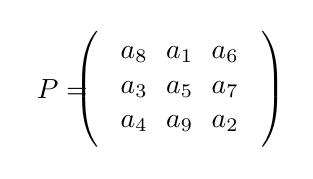
\begin{tikzpicture}
  \matrix (a) [matrix of math nodes,left delimiter=(,right delimiter=)]
{
a_8 & a_1 & a_6 \\
a_3 & a_5 & a_7 \\
a_4 & a_9 & a_2 \\
};
\node at (a.west) [xshift=-0.5cm] {$P=$};
\end{tikzpicture}
\begin{animateinline}[poster=first,autoplay, palindrome]{12}
\multiframe{29}{iangle=80+10, rdim=2.0+-0.2}{
  \begin{tikzpicture}[scale=0.1]
\fill[blue] (\iangle+45:\rdim) - - (\iangle+135:.5)- -
  (\iangle+225:\rdim)- -(\iangle+315:.5) - - cycle;
\fill[blue] (\iangle+45:.5) - - (\iangle+135:\rdim)- - (\iangle+
  225:.5)- -(\iangle+315:\rdim) - - cycle;
\end{tikzpicture} }
\end{animateinline}

\begin{animateinline}[poster=first,autoplay, palindrome]{12}
\multiframe{29}{iangle=2+1}{
  \begin{tikzpicture}[scale=1]
    \draw[domain=0:1.2] plot (\x,\x*\x) node[right] {$f(x)=x^2$};
    \draw[->] (0,0) --(1.5,0) node[right] {$x$};
    \draw[->] (0,-0.1) --(0,1.5) node[above] {$y$};
    \foreach \i in {0,1,...,\iangle} {
      \xdef \dx {1.0/\iangle}
      \xdef \x {\i *\dx} 
      \xdef \s {2}
      \pgfmathparse{\i<\iangle?1:6} 
      \let\s\pgfmathresult
      \filldraw[blue] (\x,0) -- (\x,\x*\x) --(\x+\dx/\s,\x*\x) --(\x+\dx/\s,0)--cycle;
    }
\end{tikzpicture}
}
\end{animateinline}

\begin{animateinline}[poster=first,autoplay, palindrome]{12}
\multiframe{15}{iangle=2+1}{
  \begin{tikzpicture}[scale=0.5]
    \foreach \i in {0,2,...,\iangle} {
      \xdef\dx{\i} 
      \pgfmathparse{\dx/4}
      \let\s\pgfmathresult
      \draw[blue] (0,0) circle( \s); 
    }
\end{tikzpicture}
}
\end{animateinline}

\begin{animateinline}[poster=first,autoplay, palindrome]{4}
\multiframe{13}{iangle=0+1}{
  \begin{tikzpicture}[scale=0.2]
      %\draw[blue] (0,0) circle( \s); 
  \ifthenelse{\isodd{\iangle}}{\penguin[rotate=-30,scale=0.4]; \penguin[xshift=1cm,rotate=30,scale=0.3];} { \penguin[rotate=-30,scale=0.4]; \penguin[rotate=30,xshift=1cm,scale=0.3]} 
\end{tikzpicture}
}
\end{animateinline}
\end{document}
